\documentclass[12pt, a4paper, oneside]{ctexart}
\usepackage{amsmath, amsthm, amssymb, graphicx}
\usepackage[bookmarks=true, colorlinks, citecolor=blue, linkcolor=black]{hyperref}
\usepackage[margin = 25mm]{geometry}
\usepackage{setspace}
\usepackage{listings}
\usepackage{ctex}
\usepackage{float}
\usepackage{xcolor}

\definecolor{codegreen}{rgb}{0,0.6,0}
\definecolor{codegray}{rgb}{0.5,0.5,0.5}
\definecolor{codepurple}{rgb}{0.58,0,0.82}
\definecolor{backcolour}{rgb}{0.95,0.95,0.92}

\lstdefinestyle{mystyle}{
    backgroundcolor=\color{backcolour},   
    commentstyle=\color{codegreen},
    keywordstyle=\color{magenta},
    numberstyle=\tiny\color{codegray},
    stringstyle=\color{codepurple},
    basicstyle=\ttfamily\footnotesize,
    breakatwhitespace=false,         
    breaklines=true,                 
    captionpos=b,                    
    keepspaces=true,                 
    numbers=left,                    
    numbersep=5pt,                  
    showspaces=false,                
    showstringspaces=false,
    showtabs=false,                  
    tabsize=2
}

\lstset{style=mystyle}


\title{使用隐式欧拉法求解常微分方程问题}
\date{\today}
\author{Alphabetium}
\begin{document}
\begin{spacing}{2.0}
\tableofcontents
\maketitle

\section{问题}
对于下列微分方程初值问题:
\begin{center}
$    \left\{\begin{matrix} 
        \frac{\mathrm{d}y}{\mathrm{d}x}=xy^2+2y \\  
        y(0)=-5 
      \end{matrix}\right. $
\end{center}
使用隐式欧拉法求解其在$0<x<5$时的数值解。
\section{求解方程:解析解}
透过python的sympy库求解
\begin{lstlisting}[language=Python, caption=0.1s]
    from sympy import Function, dsolve, Eq, Derivative, sin, cos, symbols
    from sympy.abc import x
    f = Function('f')
    dsolve(Derivative(f(x), x) - x * f(x)**2 -2 * f(x), f(x), ics={f(0): -5})
    
\end{lstlisting}
可以得到方程解为:
\begin{center}
    $f{\left(x \right)} = \frac{4 e^{2 x}}{- 2 x e^{2 x} + e^{2 x} - \frac{9}{5}}$
\end{center}
\section{透过三种不同方法求解微分方程}
\subsection{隐式欧拉法}
\begin{lstlisting}[language=MATLAB, caption=隐式欧拉法]
    x0 = 0;
    y0 = -5;
    a = 0;
    b = 5;
    h = 0.2;
    y = Euler_Implicit(@f, y0, a, b, h);
    
    x = linspace(a, b, length(y));
    hold on
    plot(x, y, '-o');
    plot(x,RealFunc(x),"-b");
    xlabel('x');
    ylabel('y');
    title('Numerical Solution and error');

    function y = Euler_Implicit(f, y0, a, b, h)
        n = round((b-a)/h);
        y = zeros(1, n+1);
        y(1) = y0;
        
        for i = 2:n+1
            xi = a + (i-1) * h;
            yi = y(i-1);
            for j = 1:100
                yi = y(i-1) + h * f(xi, yi);
            end
            y(i) = yi;
        end
    end
    
    function f = f(x, y)
         f= x.*y.^2 + 2.*y;
    end
    
    function ye = RealFunc(x)
        ye = (20.*exp(2.*x))./(exp(2.*x)-10.*x.*exp(2.*x)-9);
    end
    
\end{lstlisting}
其中$function ye = RealFunc(x)$部分是文章第一部分所解出的解析解;$function f = f(x, y)$部分是原方程,将$\frac{\mathrm{d}y}{\mathrm{d}x}$替换为f;
$function y = Euler\_Implicit(f, y0, a, b, h)$是函数主体,解释如下:\\
1. 根据步长 h 计算需要多少个点n,并初始化结果数组;\\
2. 将初始值赋给第一个元素;\\
3. 循环从 i=2 到 i=n+1,每次计算 xi 和 yi;\\
4. 在内部循环中进行100次迭代,利用欧拉隐式法更新 yi 的数值;\\
5. 将最终得到的 yi 赋给结果数组。\\
\begin{figure}[htbp][H]
    \centering
    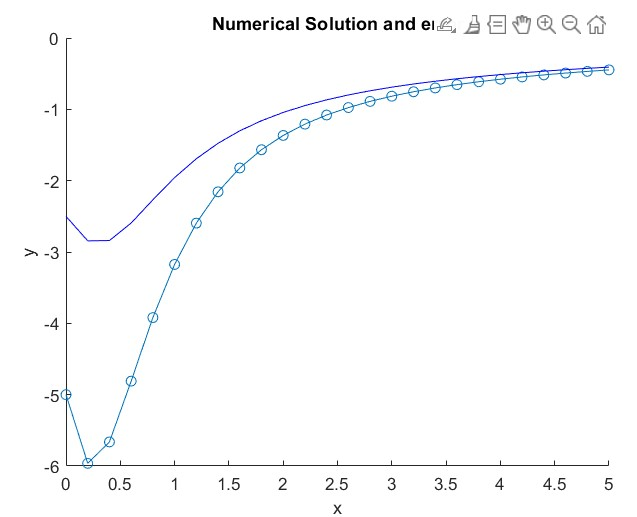
\includegraphics[width=8cm]{Eular-IM.jpg}
    \caption{隐式欧拉法}
\end{figure}

\subsection{显式欧拉法}
\begin{lstlisting}[language=MATLAB, caption=显式欧拉法]
    x0 = 0;
    y0 = -5;
    h = 0.1;
    y = Euler_Explicit(@f, y0, h);
    
    x = linspace(0, 5, length(y));
    hold on
    plot(x, y, '-o');
    plot(x,RealFunc(x),"-b");
    
    xlabel('x');
    ylabel('y');
    title('Numerical Solution and Error');
    legend('Numerical Solution');
    
    
    function y = Euler_Explicit(f, y0, h)
        t0 = 0;
        tp = 5;
        t = t0:h:tp;
        y = zeros(size(t));
        y(1) = y0;
    
        for i = 1:length(t)-1
            y(i+1) = y(i) + h * f((i+1) * h, y(i));
        end
    end
    
    function fullderi = f(x, y)
        fullderi = x.*y.^2 + 2*y;
    end
    
    function ye = RealFunc(x)
        ye = (20.*exp(2.*x))./(exp(2.*x)-10.*x.*exp(2.*x)-9);
    end    
\end{lstlisting}
$    function y = Euler\_Explicit(f, y0, h)$是函数主体,解释如下:
1.初始化变量$x_0$、$y_0$和$h$ \\
2.调用$Euler_Explicit$函数计算数值解$y$ \\
3.生成等间隔的自变量$x$ \\
4.绘制数值解曲线和真实解曲线,并添加标签、标题及图例。 \\
其中,$Euler_Explicit$函数使用欧拉显式法对微分方程进行离散化处理并求出数值近似解;$f(x,y)$为给定的微分方程右侧;$RealFunc(x)$为该微分方程的真实解。
\begin{figure}[htbp][H]
    \centering
    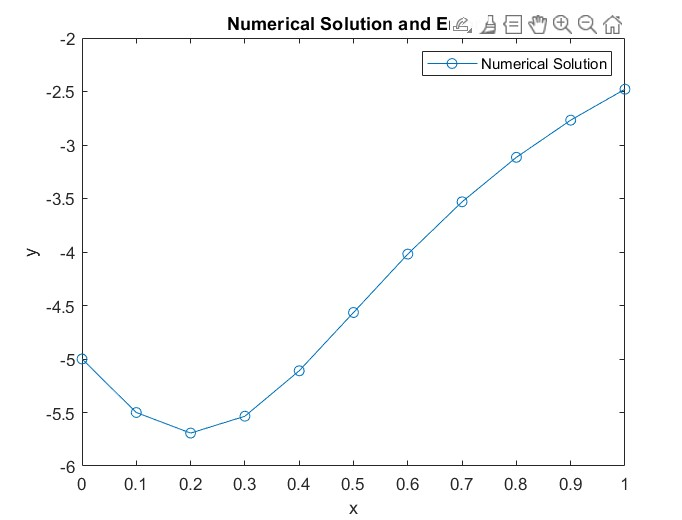
\includegraphics[width=8cm]{EE.jpg}
    \caption{显式欧拉法}
\end{figure}

\subsection{4th-order Runge-Kutta}
\begin{lstlisting}[language=MATLAB, caption=4th-order Runge-Kutta]
    y0 = -5;
    t0 = 0;
    tn = 5;
    h = 0.2;
    
    result = Runge_Kutta41(@f, t0, y0, tn, h);
    x = linspace(0, 5, length(result));
    hold on
    plot(x, result, '-o');
    plot(x,RealFunc(x),"-b");
    
    xlabel('x');
    legend();
    
    function res = Runge_Kutta41(f, t0, y0, tn, h)
        res = [y0];
        t = t0;
        for i = 1:floor((tn-t0)/h)
            k1 = f(t, res(end));
            k2 = f(t + h / 2, res(end) + h * k1 / 2);
            k3 = f(t + h / 2, res(end) + h * k2 / 2);
            k4 = f(t + h, res(end) + h * k3);
            y_next = res(end) + h*(k1 + 2 * k2 + 2 * k3 + k4)/6;
            res = [res, y_next];
            t = t + h;
        end
    end
    
    function y = f(x, y)
        y = x*y^2 + 2*y;
    end
    
    function ye = RealFunc(x)
        ye = (20.*exp(2.*x))./(exp(2.*x)-10.*x.*exp(2.*x)-9);
    end
    
\end{lstlisting}
\begin{figure}[htbp][H]
    \centering
    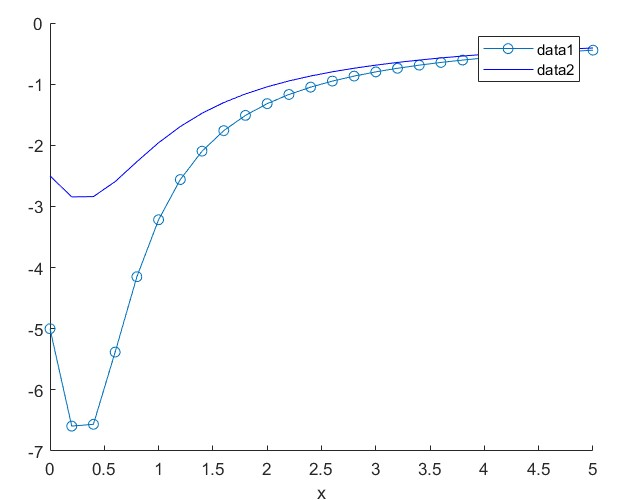
\includegraphics[width=8cm]{Runge_Kutta411.jpg}
    \caption{4th-order Runge-Kutta}
\end{figure}

这部分比较简单,主要是透过以下公式进行循环而得:
\begin{center}
    
    $    k_1 = \ f(t_n, y_n)$, \\
    $k_2 = \ f\!\left(t_n + \frac{h}{2}, y_n + h\frac{k_1}{2}\right)$, \\ 
    $k_3 = \ f\!\left(t_n + \frac{h}{2}, y_n + h\frac{k_2}{2}\right)$, \\
    $k_4 = \ f\!\left(t_n + h, y_n + hk_3\right)$.\\
    $y_{n+1} = y_n + \frac{1}{6}\left(k_1 + 2k_2 + 2k_3 + k_4 \right)$h,\\
    $t_{n+1} = t_n + h$ \\


\end{center}
\section{处理三种方法的误差-代码实现}
时间太赶实在是学不完也写不出来了,一直报错也看得不是很懂,下面的都是python,主要是分析误差。
\subsection{隐式欧拉法}
\begin{lstlisting}[language=Python, caption=隐式欧拉法]
    import numpy as np
    import matplotlib.pyplot as plt
    
    
    def Euler_Implicit(f, y0, a, b, h):
        n = round((b-a)/h)
        y = np.zeros(n+1)
        y[0] = y0
    
        for i in range(1, n+1):
            xi = a + i * h
            yi = y[i - 1]
            for j in range(10):
                yi = y[i - 1] + h * f(xi, yi)
            y[i] = yi
        
        return y
    
    
    def error(f, y0, a, b, h):
    
        def y_exact(x):
            return 20*np.exp(2*x)/(np.exp(2*x) - 10*x*np.exp(2*x) - 9)
    
        y_num = Euler_Implicit(f, y0, a, b, h)
        x = np.arange(a, b + h, h)[:len(y_num)]
        e = y_num - y_exact(x)
    
        return x, e
    
    
    def f(x, y):
        return x*y**2+2*y
    
    
    x0 = 0
    y0 = -5
    a = 0
    b = 5
    h = 0.1
    y = Euler_Implicit(f, y0, a, b, h)
    
    error_list = []
    ha = np.arange(0.1, 0.7, 0.01)
    for h in np.arange(0.1, 0.7, 0.01):
        
        y = Euler_Implicit(f, y0, a, b, h)
        x, e = error(f, y0, a, b, h)
        x = np.linspace(0, 5, len(y))
        error_list.append(e[-1])
        print(h,e[-1])
    
    
    plt.plot(ha, error_list)
    plt.xlabel('h')
    plt.ylabel('e[-1]')
    plt.title('Error vs. Step Size')
    plt.show() 
    
\end{lstlisting}
\subsection{显式欧拉法}
\begin{lstlisting}[language=Python, caption=显式欧拉法]
    import numpy as np
    import matplotlib.pyplot as plt
    
    def Euler_Explicit(f, y0, h):
        t0 = 0
        tp = 5
        t = np.arange(t0, tp+h, h)
        y = np.zeros(len(t))
        y[0] = y0
    
        for i in range(0, len(t)-1):
            y[i+1] = y[i] + h * f((i+1) * h, y[i])
        return y
    
    def error(f, y0, h):
        t0 = 0
        tp1 = 5
        
        def y_exact(x):
            return 20*np.exp(2*x)/(np.exp(2*x) - 10*x*np.exp(2*x) - 9)
    
        y_num = Euler_Explicit(f, y0, h)
        x = np.arange(t0, tp1 + h, h)
        e = y_num - y_exact(x)
    
        return x, e
        
    def f(x, y):
        return x*y**2+2*y
    x0 = 0
    y0 = -5
    
    error_list = []
    ha = np.arange(0.26, 1.5, 0.01)
    for h in np.arange(0.26, 1.5, 0.01):
        
        y = Euler_Explicit(f, y0, h)
        x, e = error(f, y0, h)
        x = np.linspace(0, 5, len(y))
        error_list.append(e[-1])
        print(h,e[-1])
    
    xdata = ha
    ydata = np.array(error_list)
    coef = np.polyfit(xdata, ydata, 2)
    f_fit = np.poly1d(coef)
    xfit = np.linspace(xdata[0], xdata[-1], 100)
    yfit = f_fit(xfit)
        
    plt.plot(ha, error_list, 'bo', label='data')
    plt.plot(xfit, yfit, 'r-', label='fit')
    plt.xlabel('h')
    plt.ylabel('e[-1]')
    plt.title('Error vs. Step Size')
    plt.legend()
    plt.show()
    plt.plot(ha, error_list)
    plt.xlabel('h')
    plt.ylabel('e[-1]')
    plt.title('Error vs. Step Size')
    plt.show()
    
\end{lstlisting}
\subsection{4th-order Runge-Kutta}
\begin{lstlisting}[language=Python, caption=4th-order Runge-Kutta]
    import numpy as np
    import matplotlib.pyplot as plt
    
    def Runge_Kutta4(f, t0, y0, tn, h):
        res = [y0]
        t = t0
        for i in range(int((tn-t0)/h)):
            k1 = f(t, res[-1])
            k2 = f(t + h / 2, res[-1] + h * k1 / 2)
            k3 = f(t + h / 2, res[-1] + h * k2 / 2)
            k4 = f(t + h, res[-1] + h * k3)
            y_next = res[-1] + h * (k1 + 2 * k2 + 2 * k3 + k4)/6
            res.append(y_next)
            t += h
        return res
    
    def f(x, y):
        return x*y**2+2*y
    
    def error(f, y0, t0, tn, h):
    
        def y_exact(t):
            return 20*np.exp(2*x)/(np.exp(2*x) - 10*x*np.exp(2*x) - 9)
    
        y_num = Runge_Kutta4(f, t0, y0, tn, h)
        t = np.arange(t0, tn + h, h)
        e = y_num - y_exact(t)
    
        return t, e
    
    y0 = -5
    t0 = 0
    tn = 5
    h = 0.1
    
    result = Runge_Kutta4(f, t0, y0, tn, h)
    x = np.linspace(0, 5, len(result))
    plt.plot(x, result, '-o',label='Numerical Solution')
    
    t, e = error(f, y0, t0, tn, h)
    
    plt.plot(t, e, '-o', label='Error')
    
    plt.xlabel('t')
    plt.title('Numerical Solution and Error')
    plt.legend()
    plt.show()
    
\end{lstlisting}
\section{处理三种方法的误差-比较}
\begin{figure}[H]
    \begin{minipage}[t]{0.5\linewidth}
        \centering
        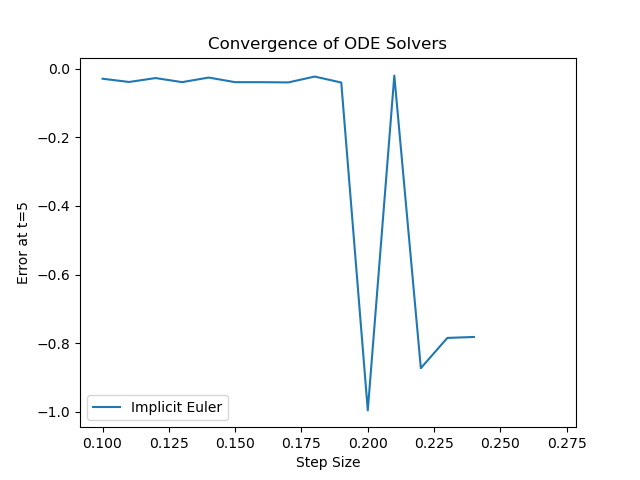
\includegraphics[scale=0.3]{EIM-ddd.png}
        \caption{隐式欧拉法的误差}
        \label{fig:side:a}
      \end{minipage}%
      \begin{minipage}[t]{0.5\linewidth}
        \centering
        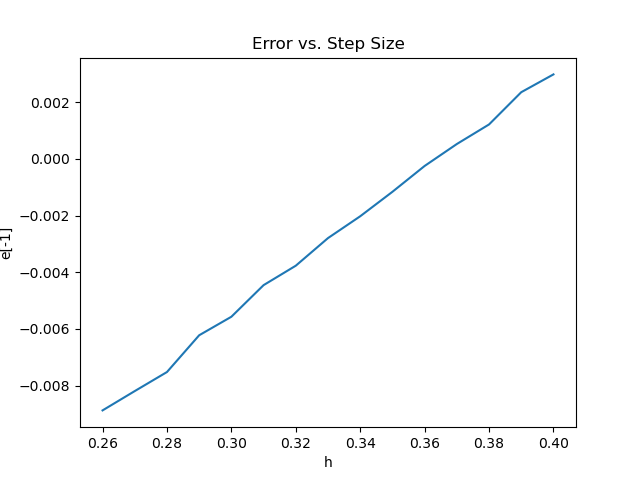
\includegraphics[scale=0.3]{EE-ddd.png}
        \caption{显式欧拉法的误差}
        \label{fig:side:b}
      \end{minipage}
      \begin{minipage}[t]{0.5\linewidth}
        \centering
        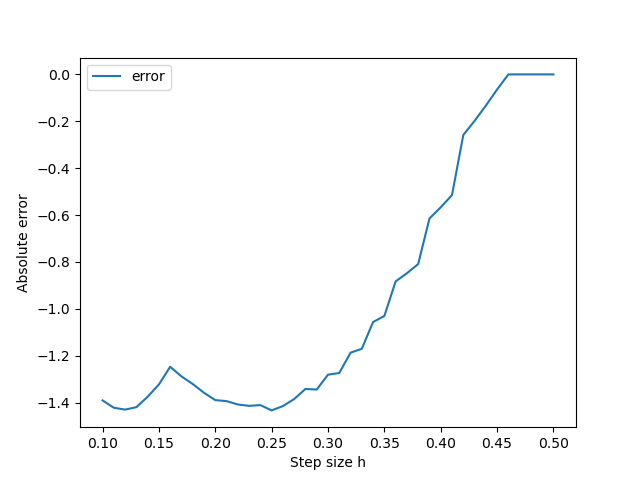
\includegraphics[scale=0.3]{Runge_Kutta4 ddd.png}
        \caption{4th-order Runge-Kutta的误差}
        \label{fig:side:b}
      \end{minipage}
\end{figure}

我将数据处理的档案加到附件里
输出结果为:
\begin{center}
    EE.txt: 最接近 0 的值是 [0.26, -0.008873641307191593],其距离为 0.2688736413071916。\\
    EIM.txt: 最接近 0 的值是 [0.1, -0.03759539961851743],其距离为 0.13759539961851744。\\
    runge.txt: 最接近 0 的值是 [0.44999999999999984, -0.06431906956574363],其距离为 0.5143190695657435。
\end{center}
比较上面三张图片及处理完的数据可以看出隐式欧拉法在步长的选取上可以选择的精度最小,说明在这三种方法中最为精确。

\end{spacing}{}

\end{document}
